%%%%%%%% Final Report -- PagedAttention in MiniTorch %%%%%%%%%

\documentclass{article}

\usepackage{microtype}
\usepackage{graphicx}
\usepackage{subfigure}
\usepackage{booktabs}
\usepackage{amsmath}
\usepackage{xcolor}
\usepackage{listings}
\usepackage{hyperref}

\newcommand{\theHalgorithm}{\arabic{algorithm}}

\usepackage[accepted]{mlsys2024}

\graphicspath{{./}}

\lstset{
  basicstyle=\ttfamily\scriptsize,
  columns=fullflexible,
  keepspaces=true,
  breaklines=true,
  frame=single,
  framerule=0.25pt,
  xleftmargin=0.3em,
  xrightmargin=0.3em,
  aboveskip=0.35em,
  belowskip=0.35em
}

\mlsystitlerunning{Final Report: PagedAttention in MiniTorch}

\begin{document}

\twocolumn[
\mlsystitle{PagedAttention in MiniTorch: KV Cache Efficiency, Prefix Reuse, and Memory Sharing}

\mlsyssetsymbol{equal}{*}

\begin{mlsysauthorlist}
\mlsysauthor{NingRui Yang}{affil}
\mlsysauthor{Yixiang Dai}{affil}
\end{mlsysauthorlist}

\mlsysaffiliation{affil}{ECE, Carnegie Mellon University, Pittsburgh, PA, US}

\mlsyskeywords{PagedAttention, KV Cache, Prefix Caching, MiniTorch, CUDA, LLM Inference}

\vskip 0.25in

\begin{abstract}
Large language model serving is often limited less by attention arithmetic than by the memory reserved for the key-value (KV) cache during autoregressive generation.  A contiguous KV cache is easy to index, but it reserves a worst-case slab per request and wastes capacity whenever prompts and generated lengths are shorter than the cap.  We implement PagedAttention in MiniTorch to expose the core systems idea behind vLLM in a compact educational codebase: store KV tensors in fixed-size physical blocks, translate logical token positions through per-sequence block tables, and share complete prefix blocks using reference counts.  Our implementation includes a Python block manager, prefix-cache and branch-sharing APIs, a transformer integration, a CUDA decode kernel and runtime, a contiguous-KV baseline, and a benchmark suite.  On a realistic non-aligned workload, block-granular allocation reaches 96.6\% KV efficiency versus 23.4\% for worst-case static reservation and 46.8\% for a realistic static cap.  Under a fixed KV budget, it supports up to 2.00x more concurrent short prompts, gives up to 1.90x faster cached-prefix prefill, and reduces KV blocks by up to 78--79\% in parallel-sampling and beam-style branching simulations.
\end{abstract}
]

\printAffiliationsAndNotice{}

% ============================================================================
\section{Introduction and Motivation}

Autoregressive LLM inference repeatedly appends one token to each active request.  To avoid recomputing all previous attention states, serving systems store each layer's key and value vectors in a KV cache.  The cache grows linearly with sequence length, number of layers, and hidden size:
\[
\text{bytes/token} = 2 \cdot L \cdot H \cdot d_h \cdot \text{sizeof(dtype)}.
\]
At serving scale, these bytes directly determine how many requests fit on a GPU.

The simplest allocation strategy reserves a contiguous KV slab for every active request up to a maximum context or admission cap.  That strategy is operationally convenient but wasteful: most requests terminate before the cap, prompt lengths are not aligned with allocator boundaries, and multi-output generation duplicates the same prompt cache.  These effects reduce effective batch size even when compute units are idle.

PagedAttention~\cite{kwon2023efficient} changes the memory contract.  Instead of requiring each request's KV cache to be physically contiguous, it partitions the cache into fixed-size blocks and uses a block table to map logical token positions to physical blocks.  This project reimplements that idea inside MiniTorch, trading production-level optimization for a readable implementation that makes the allocator, cache sharing, CUDA path, and experimental tradeoffs explicit.

Our contributions are:
\begin{enumerate}
    \item a reference-counted \texttt{BlockManager} with block tables, fragmentation accounting, prefix-cache lookup/publication, fork and clone APIs, and KV memory accounting;
    \item a MiniTorch decoder integration that supports prefill, decode, prefix reuse, and generation over paged KV blocks;
    \item a custom CUDA V1-style decode kernel and device-resident runtime buffers for non-contiguous KV lookup;
    \item a contiguous-KV baseline and six benchmark families covering memory efficiency, capacity, decode speed, prefix prefill, parallel sampling, and beam-style branch sharing.
\end{enumerate}

% ============================================================================
\section{Related Work and Background}

\textbf{PagedAttention and vLLM.}  Kwon et al.~\cite{kwon2023efficient} introduced PagedAttention as the central memory manager in vLLM.  Their production system combines block tables, continuous batching, prefix/block sharing, scheduling, and highly optimized CUDA kernels.  Our work follows the same block-granular KV storage abstraction, but differs in purpose and scope: we implement it in MiniTorch with small, inspectable Python and CUDA components, and our measurements isolate the allocator effects rather than claiming production serving throughput.

\textbf{Attention kernels.}  FlashAttention~\cite{dao2022flashattention} and FlashAttention-2~\cite{dao2023flashattention2} reduce attention IO by tiling softmax computation, while FlashInfer~\cite{ye2025flashinfer} provides modern serving-oriented attention kernels, including paged layouts.  These works optimize the attention computation path.  Our project instead emphasizes KV residency policy: how cache bytes are reserved, reused, shared, and reclaimed.  We implement a simple V1 kernel to validate non-contiguous lookup, not to match FlashAttention-class throughput.

\textbf{Serving frameworks and OS analogy.}  Systems such as Hugging Face Text Generation Inference~\cite{huggingface2023tgi} and TensorRT-LLM~\cite{tensorrtllm2024} also use KV-cache management techniques inspired by PagedAttention.  The abstraction is analogous to virtual memory paging~\cite{silberschatz2018os}: logical token blocks are virtual pages, physical KV blocks are page frames, and the block table is a page table.  MiniTorch~\cite{rush2020minitorch} gives us a small enough framework to rebuild these pieces directly.

% ============================================================================
\section{Methodology}

We organized the project around four research questions.
\begin{itemize}
    \item \textbf{RQ1:} How much reserved KV memory can block-granular allocation recover under non-aligned request lengths?
    \item \textbf{RQ2:} Under a fixed KV-block budget, how much additional concurrency does paged allocation allow?
    \item \textbf{RQ3:} How much do prefix caching and branch sharing reduce repeated work and duplicated KV state?
    \item \textbf{RQ4:} What does a minimal CUDA implementation need in order to compute attention over non-contiguous cache blocks correctly?
\end{itemize}

\subsection{Block-Granular KV Allocation}

The allocator owns a global key cache and value cache for each layer, shaped \texttt{(num\_blocks, block\_size, n\_head, head\_dim)}.  A request receives a \texttt{BlockTable}; token \(t\) is translated by \(\lfloor t/B\rfloor\) and \(t \bmod B\), where \(B\) is the block size.  Allocation is demand driven: prefill allocates \(\lceil T/B\rceil\) blocks for a prompt of length \(T\), decode appends into the current tail block when possible, and retired requests decrement reference counts and return zero-reference blocks to the free list.

Internal fragmentation is the unused tail space inside allocated blocks.  This creates a real block-size tradeoff: smaller blocks reduce tail waste, while larger blocks reduce table size and may improve locality.  Our fragmentation and capacity experiments deliberately use non-aligned lengths so this tradeoff is visible.

\subsection{Prefix Cache and Branch Sharing}

The prefix cache shares only complete blocks.  After prefill finishes for all layers, \texttt{publish\_sequence\_prefix\_blocks} computes a hash chain over the full logical blocks and maps each hash to its physical block id.  Later requests call \texttt{lookup\_prefix\_blocks}; matching blocks are inserted into the new request's block table and their reference counts are incremented.  Partial tail blocks are not shared, which keeps mutation rules simple.

Branching workloads use the same ownership mechanism.  \texttt{fork\_sequence} models a paged branch by sharing the parent's existing block table and allocating new blocks only as children diverge.  \texttt{clone\_sequence} models a naive baseline that physically duplicates the prompt KV for each output.  This lets us quantify memory effects for parallel sampling and beam-like generation without implementing a full scheduler.

\subsection{CUDA Decode Path}

The CUDA kernel assigns one thread block to each \((\text{sequence}, \text{head})\) pair.  It performs three passes: compute \(q \cdot k\) logits through block-table lookups, apply a stable softmax with warp reductions, and accumulate weighted values.  The host runtime keeps cache, query, block-table, context-length, and output buffers on the device, and exposes C-callable update methods used from Python.

Our kernel is intentionally simple.  It is useful for correctness and for teaching the translation from logical tokens to physical KV blocks, but it lacks vLLM-style template specialization, coalesced cache layouts, online softmax, and V2 multi-block decomposition for long contexts.

\subsection{Baselines}

We use two baselines.  The no-cache baseline re-runs the full prompt at each decode step, which highlights the algorithmic benefit of caching but is not a fair serving implementation.  The contiguous-KV baseline wraps the same \texttt{PagedDecoderLM} weights with HuggingFace-style preallocated K/V arrays shaped \texttt{(max\_batch, n\_head, max\_seq\_len, head\_dim)}.  It avoids recomputing the prompt but still pays static contiguous reservation.

% ============================================================================
\section{Implementation Details and Code Snippets}

The implementation spans \texttt{minitorch/block\_manager.py}, \texttt{minitorch/transformer.py}, \texttt{minitorch/paged\_attention.py}, \texttt{src/paged\_attention.cu}, \texttt{project/contiguous\_kv\_baseline.py}, and the benchmark scripts in \texttt{project/}.  Figure~\ref{fig:snippets} shows the three most important mechanics: prefix-backed allocation, the CUDA block-table translation, and the runtime's device-resident cache updates.

\begin{figure*}[t]
\centering
\begin{minipage}[t]{0.32\textwidth}
\begin{lstlisting}[language=Python]
def allocate_sequence_with_prefix(seq_id, num_tokens, prefix_blocks):
    table = BlockTable(seq_id)
    for bid in prefix_blocks:
        table.append_block(bid)
        blocks[bid].ref_count += 1

    remaining = num_tokens - len(prefix_blocks) * block_size
    for _ in range(ceil(remaining / block_size)):
        block = allocate_block()
        table.append_block(block.block_id)
        block.num_filled = min(remaining, block_size)
        remaining -= block.num_filled
\end{lstlisting}
\end{minipage}\hfill
\begin{minipage}[t]{0.32\textwidth}
\begin{lstlisting}[language=C]
int logical_block = token_idx / block_size;
int slot = token_idx % block_size;
int physical_block = seq_block_table[logical_block];

const float* k = key_cache
  + physical_block * (block_size * n_head * head_dim)
  + slot * (n_head * head_dim)
  + head_idx * head_dim;
\end{lstlisting}
\end{minipage}\hfill
\begin{minipage}[t]{0.32\textwidth}
\begin{lstlisting}[language=C]
void paged_attention_runtime_update_slot(
    void* handle, int block_id, int slot_idx,
    const float* key_host, const float* value_host) {
  size_t off = ((size_t)block_id * block_size + slot_idx)
             * n_head * head_dim;
  cudaMemcpy(d_key_cache + off, key_host, slot_bytes,
             cudaMemcpyHostToDevice);
  cudaMemcpy(d_value_cache + off, value_host, slot_bytes,
             cudaMemcpyHostToDevice);
}
\end{lstlisting}
\end{minipage}
\caption{Representative implementation snippets.  Left: cached prefix blocks are reused by reference and only suffix blocks are allocated.  Middle: the CUDA kernel translates logical token positions into physical cache addresses.  Right: the runtime updates individual block slots without reallocating the full cache.}
\label{fig:snippets}
\end{figure*}

The transformer integration separates prefill and decode.  During prefill, the model checks prefix-cache hits before allocating blocks; hit groups compute only suffix tokens while attending to cached prefix K/V.  During decode, each active sequence appends one logical token, writes the new K/V into its physical block slot, and calls paged attention over the full cached context.

A major engineering issue was CUDA context ownership.  MiniTorch uses Numba/PyCUDA driver-API paths, PyTorch uses the CUDA runtime API, and our shared library also uses runtime calls.  The fix was to compile with shared \texttt{libcudart}, initialize the runtime early, and make driver-API imports lazy.  Without this, runtime calls could fail after Numba had initialized a separate context.

% ============================================================================
\section{Experiments}

\subsection{Setup}

The final benchmark suite in \texttt{project/run\_rigorous\_benchmark.py} runs six experiments and plots them with \texttt{project/plot\_rigorous\_figures.py}.  Unless otherwise stated, the report-grade configuration uses \texttt{n\_embd=512}, \texttt{n\_head=8}, \texttt{n\_layers=4}, \texttt{block\_size=16}, \texttt{num\_kv\_blocks=512}, and one warmup plus three timed trials for timing experiments.  Correctness is checked by unit tests and by benchmark rows that compare paged attention against reference outputs.

\subsection{Memory Efficiency and Capacity}

Figure~\ref{fig:memory_capacity} reports the central allocator result.  For the realistic non-aligned workload \([48,67,112,160,256,80,35,200]\), paged allocation reserves only the blocks needed for live tokens and reaches 96.6\% KV efficiency.  Worst-case static reservation at \texttt{n\_positions=512} is only 23.4\% efficient; a more realistic static cap at the maximum observed length is 46.8\% efficient.  The capacity curve then fixes the KV budget and asks how many concurrent sequences fit.  Paged allocation supports up to 2.00x more short prompts than the static \texttt{seq\_len+32} cap and remains 1.14x better at 256 tokens.

\begin{figure*}[t]
\centering
\subfigure[Reserved versus live KV bytes.]{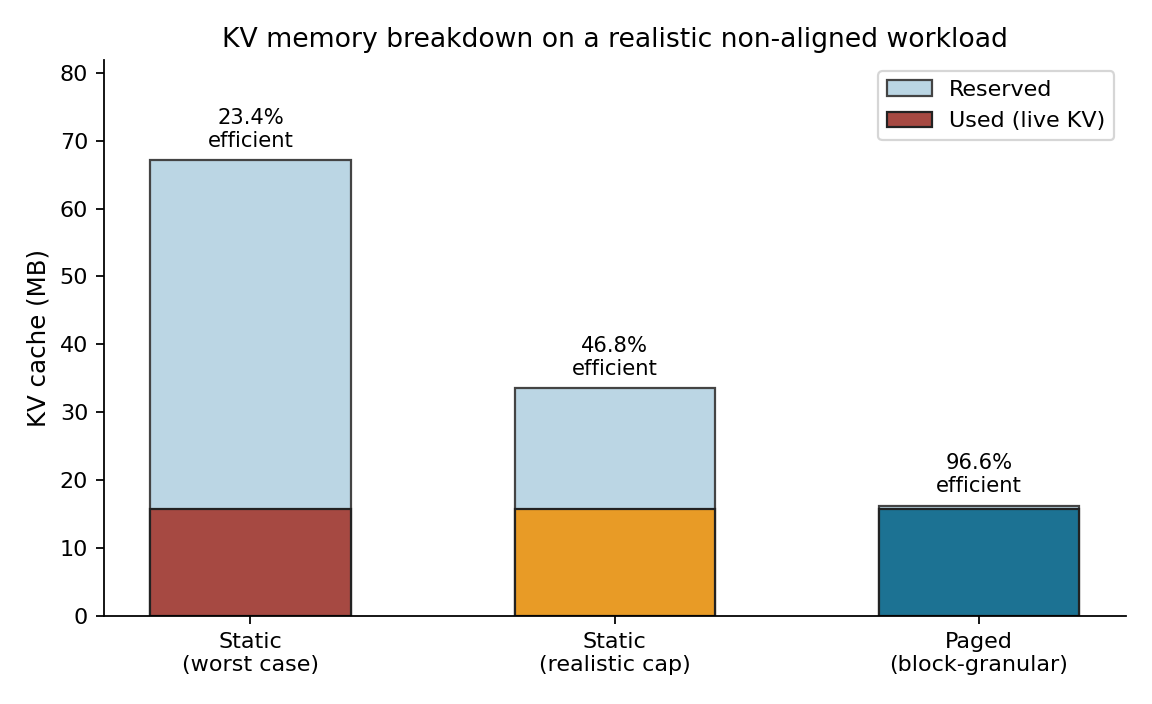
\includegraphics[width=0.48\textwidth]{figure1.png}}
\subfigure[Max concurrent sequences under a fixed KV budget.]{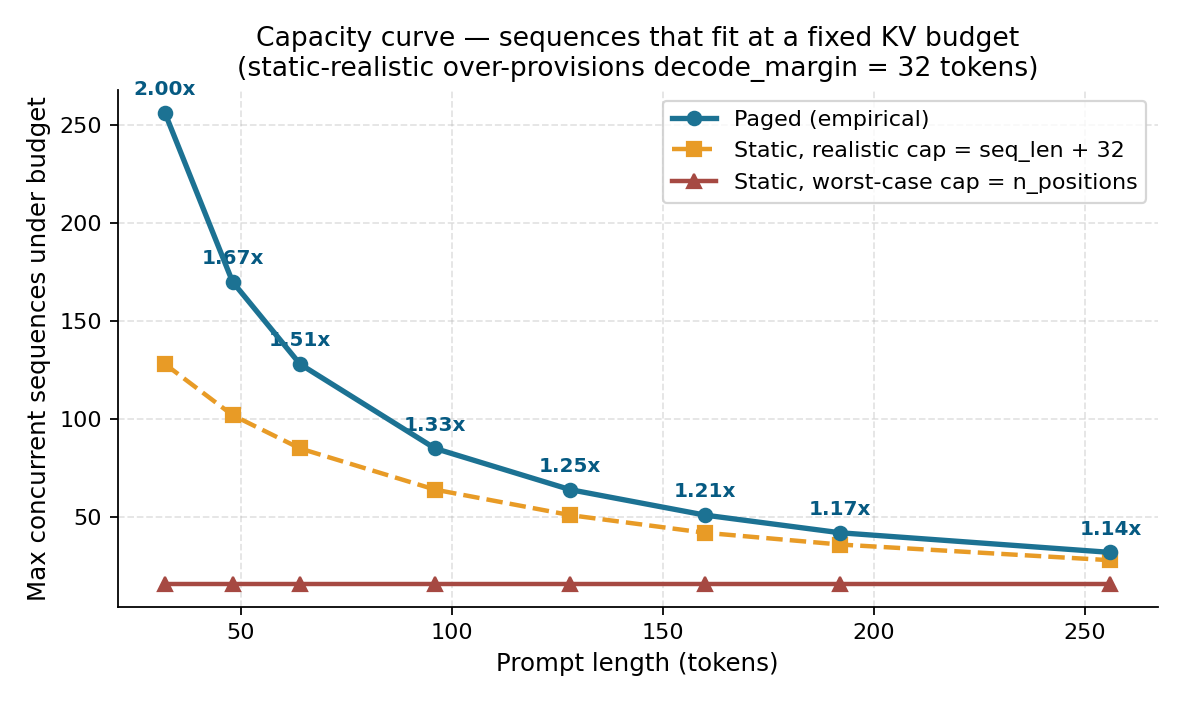
\includegraphics[width=0.48\textwidth]{figure2.png}}
\caption{Paged allocation converts worst-case per-request reservation into block-granular demand allocation.}
\label{fig:memory_capacity}
\end{figure*}

\subsection{Decode and Prefix Timing}

Decode timing compares paged KV against both no-cache re-prefill and contiguous KV.  Paged decode is consistently faster than the no-cache baseline because it reuses K/V rather than recomputing the full prefix.  Compared with the contiguous-KV baseline, the result is closer and sometimes favors the simpler contiguous path; this is expected because our educational kernel and Python runtime prioritize clarity over memory-coalesced production performance.  We therefore treat Figure~\ref{fig:timing} as evidence that caching works and as a reminder that allocator wins do not automatically imply a faster kernel.

Prefix caching shows the clearest timing benefit.  Requests with shared prompt prefixes reuse full cached blocks and compute only the suffix.  At requested shared-prefix fractions of 0\%, 25\%, 50\%, and 75\%, the measured prefill speedups are 1.36x, 1.80x, 1.76x, and 1.90x respectively.  The 0\% case is not a contradiction: with block-level cache behavior and benchmark overheads, even small allocator/runtime effects can shift short prefill timings; the main trend is that more full-block sharing reduces work.

\begin{figure*}[t]
\centering
\subfigure[End-to-end wall time for paged, contiguous KV, and no-cache decode.]{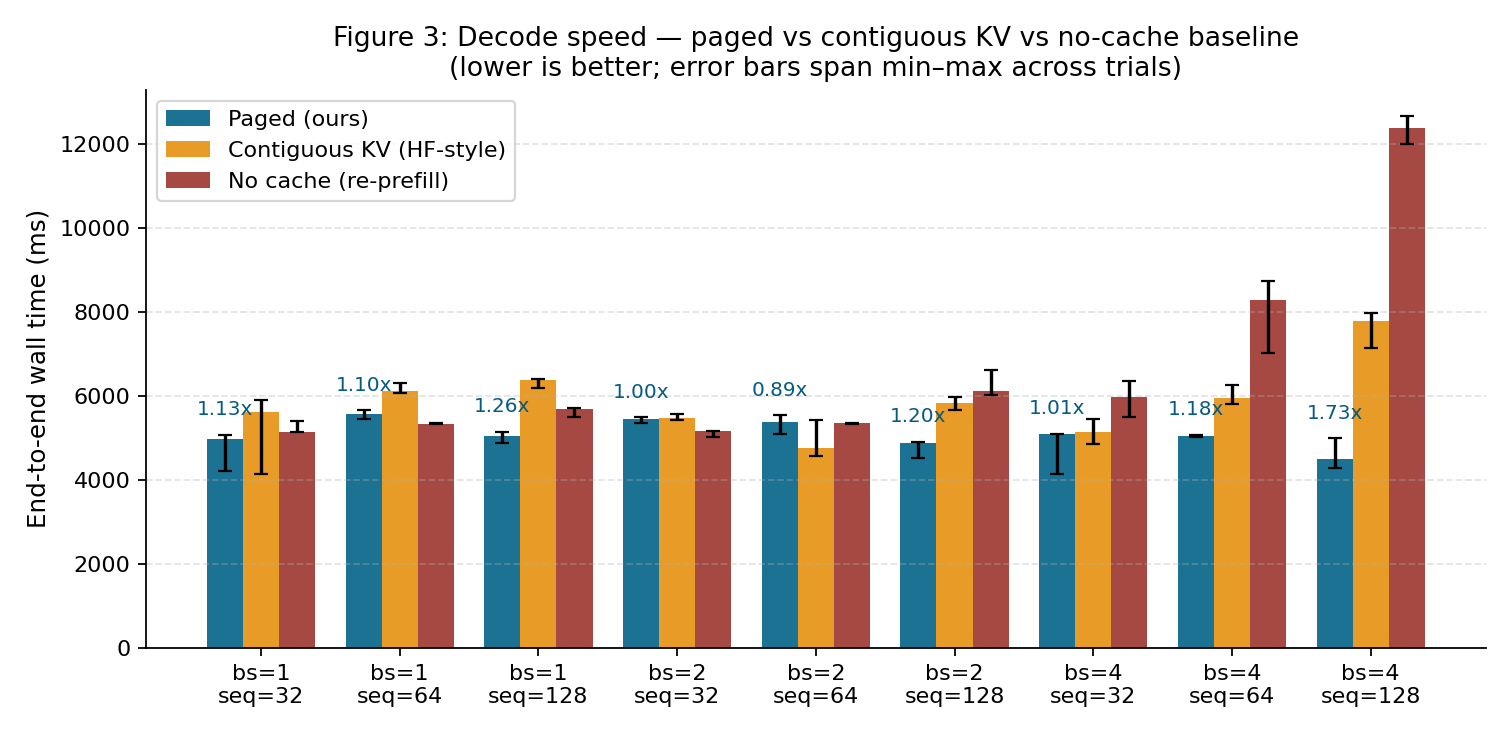
\includegraphics[width=0.48\textwidth]{figure3.png}}
\subfigure[Prefix-cache prefill speedup at varying shared fractions.]{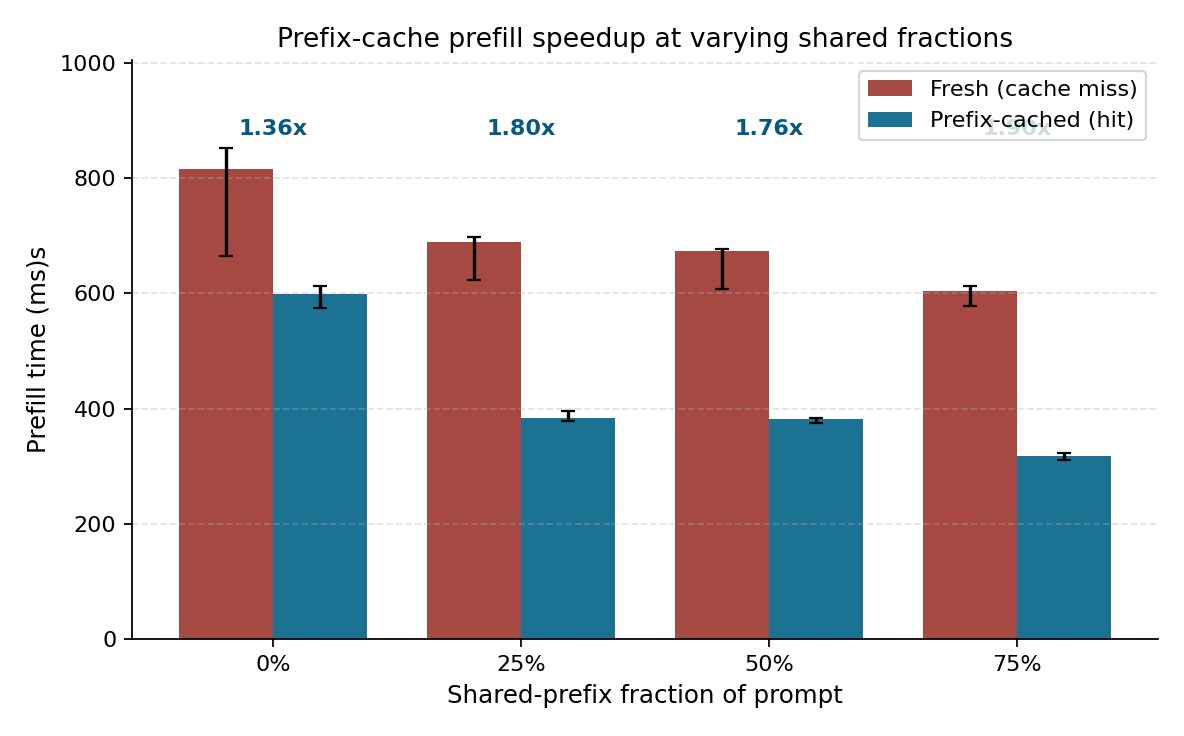
\includegraphics[width=0.48\textwidth]{figure4.png}}
\caption{Timing experiments separate caching benefits from CUDA/kernel quality.  Error bars show min--max across timed trials where available.}
\label{fig:timing}
\end{figure*}

\subsection{Branching Memory}

Multi-output generation is a natural fit for block sharing.  In parallel sampling, several completions share one prompt and diverge only after the prompt.  In beam-style search, surviving hypotheses can also share a generated trunk before the final branch.  Figure~\ref{fig:branching} compares naive cloning with paged fork semantics.  Parallel sampling saves 33--78\% of KV blocks depending on prompt length and number of outputs.  The beam-style simulation saves 33--79\% at peak and even more after pruning because the prompt and winning trunk are shared.

\begin{figure*}[t]
\centering
\subfigure[Parallel-sampling KV blocks.]{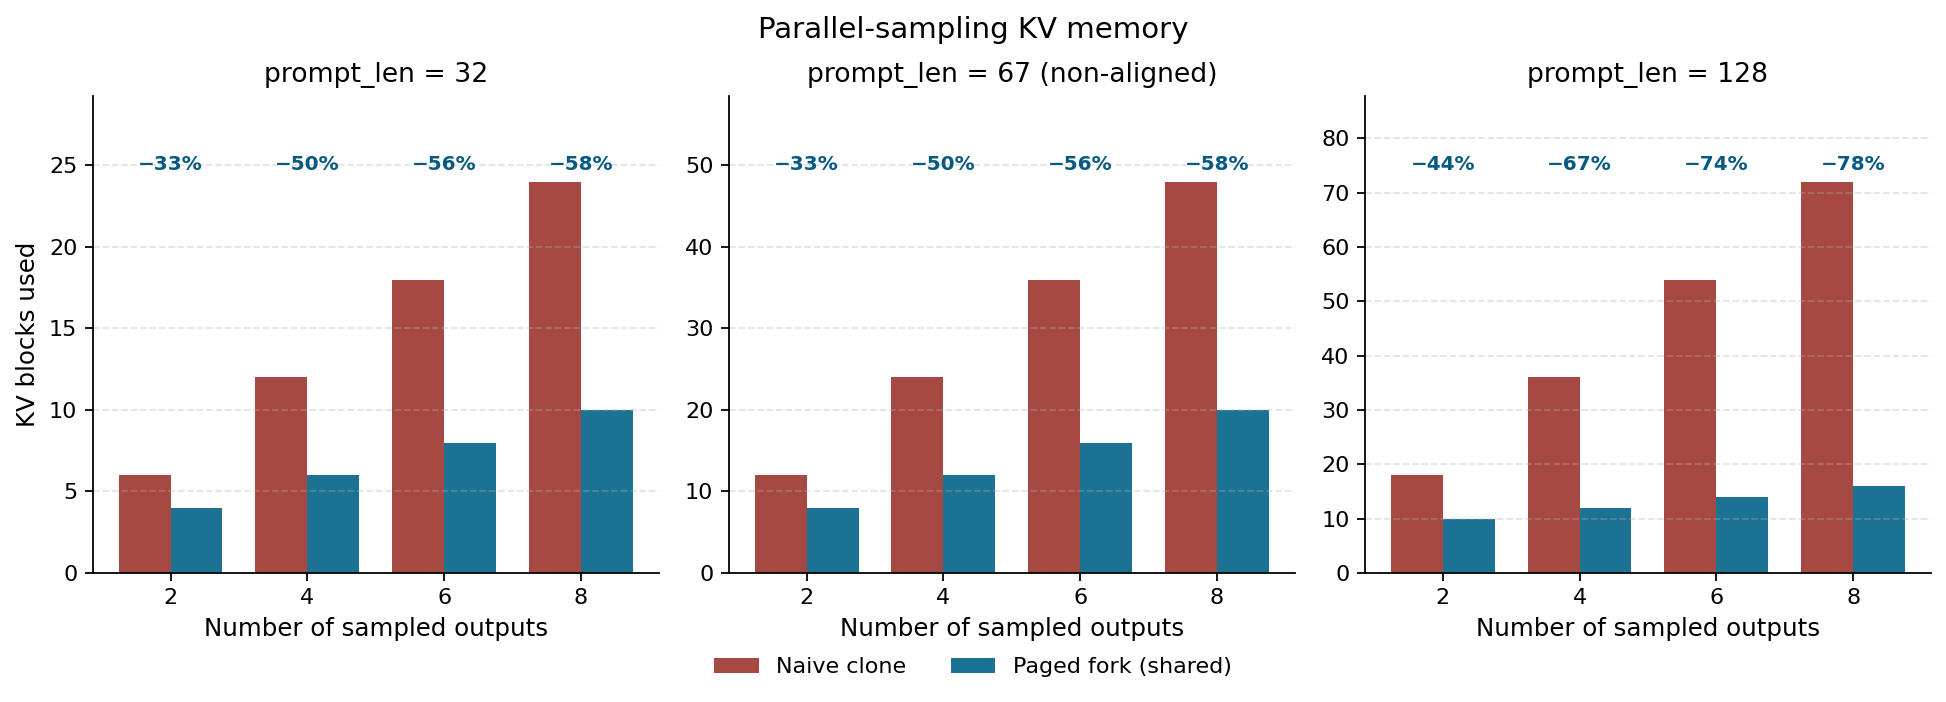
\includegraphics[width=0.48\textwidth]{figure5.png}}
\subfigure[Beam-style KV blocks.]{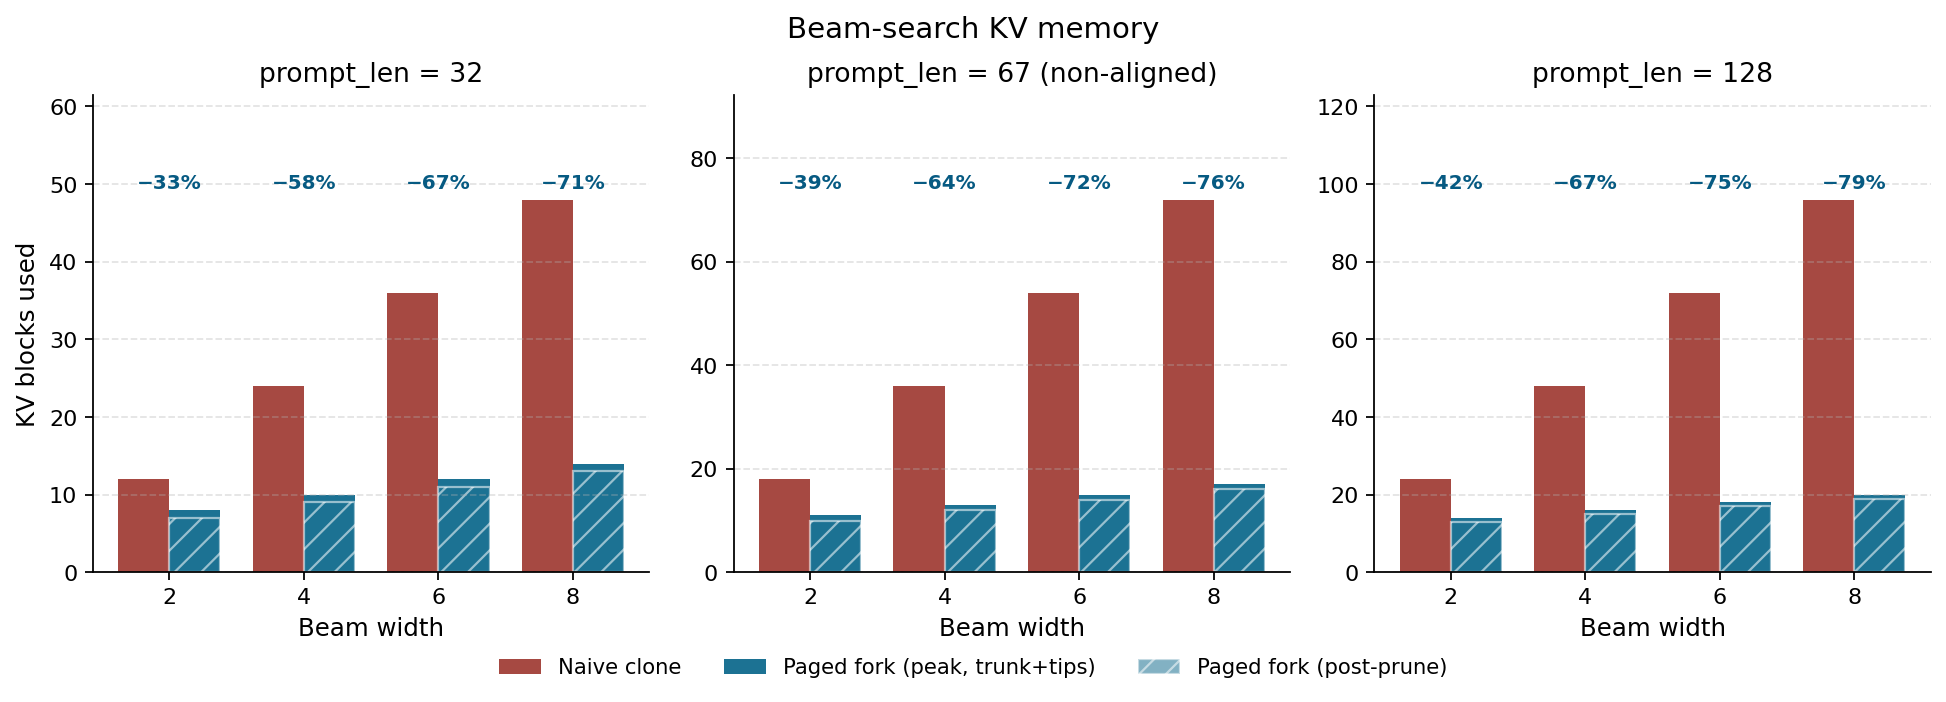
\includegraphics[width=0.48\textwidth]{figure6.png}}
\caption{Reference-counted block tables make prompt and trunk sharing a memory policy rather than a model change.}
\label{fig:branching}
\end{figure*}

% ============================================================================
\section{Analysis, Ablations, and Findings}

\textbf{Block size controls allocator waste.}  The dedicated fragmentation sweep confirms the expected tradeoff.  For sequence length 33, internal fragmentation is 17.5\% with block size 8 and 31.3\% with block size 16.  For longer or better-aligned lengths such as 100 and 130, the gap narrows.  Thus, block size should be chosen with both workload length distribution and kernel/table overhead in mind.

\textbf{Memory gains are stronger than speed gains in this prototype.}  Paged allocation dramatically improves KV efficiency and fixed-budget capacity, but our decode timing is limited by Python/MiniTorch overhead and a simple CUDA path.  This matches the project goal: validate the systems abstraction in a compact framework, not reproduce vLLM throughput.

\textbf{Sharing multiplies the allocator benefit.}  Prefix caching, parallel sampling, and beam sharing all use the same block-table/reference-count mechanism.  This is the main design lesson: once requests store mappings instead of private slabs, reuse policies become metadata updates rather than tensor copies.

\textbf{What did not work as production evidence.}  No-cache decode is useful pedagogically but overstates speedup against a real serving engine.  We therefore added the contiguous-KV baseline to distinguish caching benefits from paging benefits.  Similarly, the branch experiments are allocator simulations, not complete parallel sampling or beam-search schedulers.

% ============================================================================
\section{Conclusion and Discussion}

This project shows that PagedAttention's core idea can be rebuilt in a small teaching framework while preserving the most important systems behaviors.  Block-granular KV allocation raises realistic-workload efficiency to 96.6\%, doubles short-prompt capacity under a fixed KV budget, accelerates cached-prefix prefill, and makes multi-output KV sharing cheap.  The main takeaway is that memory residency policy is a first-class serving optimization: it can improve admission capacity, reuse, and branching efficiency without changing model weights or attention semantics.

Known limitations remain.  The CUDA kernel is a readable V1 implementation, not a production kernel.  The cache layout is not optimized for coalescing, there is no V2 decomposition for very long contexts, and some runtime paths still perform host-device transfers that a production server would avoid.  The prefix cache shares only complete blocks and lacks a full production eviction/scheduler policy.  Finally, our report-grade branch experiments model allocator behavior, not complete request scheduling or quality-aware beam search.  Future work would add GPU-resident end-to-end serving, online softmax and templated kernels, Nsight profiling, FP16/BF16 support, and a scheduler that combines paged allocation with admission control.

% ============================================================================
\section{Team Member Contributions}

\textbf{NingRui Yang} implemented and documented the allocator and model integration: the \texttt{BlockManager}, \texttt{KVBlock}, \texttt{BlockTable}, fragmentation and memory accounting, prefix-cache publication/lookup, and fork/clone sharing paths in \texttt{minitorch/block\_manager.py}; the prefill/decode/generation integration in \texttt{minitorch/transformer.py}; and project documentation under \texttt{docs/} explaining the block manager, memory accounting, prefix cache, and usage workflow.

\textbf{Yixiang Dai} implemented and evaluated the CUDA and benchmarking paths: the V1 paged-attention kernel and runtime functions in \texttt{src/paged\_attention.cu}; the Python/CUDA wrapper path used by MiniTorch; the contiguous-KV comparison baseline in \texttt{project/contiguous\_kv\_baseline.py}; and the benchmark/plotting scripts \texttt{project/run\_benchmark.py}, \texttt{project/run\_rigorous\_benchmark.py}, \texttt{project/plot.py}, and \texttt{project/plot\_rigorous\_figures.py} that produced the final report figures.

Both members collaborated on correctness tests, debugging the CUDA runtime/driver context issue, interpreting benchmark results, building the poster, and writing this final report.

\bibliography{example_paper}
\bibliographystyle{mlsys2024}

\end{document}